\documentclass[twoside]{book}

% Packages required by doxygen
\usepackage{calc}
\usepackage{doxygen}
\usepackage{graphicx}
\usepackage[utf8]{inputenc}
\usepackage{makeidx}
\usepackage{multicol}
\usepackage{multirow}
\usepackage{textcomp}
\usepackage[table]{xcolor}

% Font selection
\usepackage[T1]{fontenc}
\usepackage{mathptmx}
\usepackage[scaled=.90]{helvet}
\usepackage{courier}
\usepackage{amssymb}
\usepackage{sectsty}
\renewcommand{\familydefault}{\sfdefault}
\allsectionsfont{%
  \fontseries{bc}\selectfont%
  \color{darkgray}%
}
\renewcommand{\DoxyLabelFont}{%
  \fontseries{bc}\selectfont%
  \color{darkgray}%
}

% Page & text layout
\usepackage{geometry}
\geometry{%
  a4paper,%
  top=2.5cm,%
  bottom=2.5cm,%
  left=2.5cm,%
  right=2.5cm%
}
\tolerance=750
\hfuzz=15pt
\hbadness=750
\setlength{\emergencystretch}{15pt}
\setlength{\parindent}{0cm}
\setlength{\parskip}{0.2cm}
\makeatletter
\renewcommand{\paragraph}{%
  \@startsection{paragraph}{4}{0ex}{-1.0ex}{1.0ex}{%
    \normalfont\normalsize\bfseries\SS@parafont%
  }%
}
\renewcommand{\subparagraph}{%
  \@startsection{subparagraph}{5}{0ex}{-1.0ex}{1.0ex}{%
    \normalfont\normalsize\bfseries\SS@subparafont%
  }%
}
\makeatother

% Headers & footers
\usepackage{fancyhdr}
\pagestyle{fancyplain}
\fancyhead[LE]{\fancyplain{}{\bfseries\thepage}}
\fancyhead[CE]{\fancyplain{}{}}
\fancyhead[RE]{\fancyplain{}{\bfseries\leftmark}}
\fancyhead[LO]{\fancyplain{}{\bfseries\rightmark}}
\fancyhead[CO]{\fancyplain{}{}}
\fancyhead[RO]{\fancyplain{}{\bfseries\thepage}}
\fancyfoot[LE]{\fancyplain{}{}}
\fancyfoot[CE]{\fancyplain{}{}}
\fancyfoot[RE]{\fancyplain{}{\bfseries\scriptsize Generated on Sun Nov 1 2015 17\-:50\-:53 for My Project by Doxygen }}
\fancyfoot[LO]{\fancyplain{}{\bfseries\scriptsize Generated on Sun Nov 1 2015 17\-:50\-:53 for My Project by Doxygen }}
\fancyfoot[CO]{\fancyplain{}{}}
\fancyfoot[RO]{\fancyplain{}{}}
\renewcommand{\footrulewidth}{0.4pt}
\renewcommand{\chaptermark}[1]{%
  \markboth{#1}{}%
}
\renewcommand{\sectionmark}[1]{%
  \markright{\thesection\ #1}%
}

% Indices & bibliography
\usepackage{natbib}
\usepackage[titles]{tocloft}
\setcounter{tocdepth}{3}
\setcounter{secnumdepth}{5}
\makeindex

% Hyperlinks (required, but should be loaded last)
\usepackage{ifpdf}
\ifpdf
  \usepackage[pdftex,pagebackref=true]{hyperref}
\else
  \usepackage[ps2pdf,pagebackref=true]{hyperref}
\fi
\hypersetup{%
  colorlinks=true,%
  linkcolor=blue,%
  citecolor=blue,%
  unicode%
}

% Custom commands
\newcommand{\clearemptydoublepage}{%
  \newpage{\pagestyle{empty}\cleardoublepage}%
}


%===== C O N T E N T S =====

\begin{document}

% Titlepage & ToC
\hypersetup{pageanchor=false}
\pagenumbering{roman}
\begin{titlepage}
\vspace*{7cm}
\begin{center}%
{\Large My Project }\\
\vspace*{1cm}
{\large Generated by Doxygen 1.8.6}\\
\vspace*{0.5cm}
{\small Sun Nov 1 2015 17:50:53}\\
\end{center}
\end{titlepage}
\clearemptydoublepage
\tableofcontents
\clearemptydoublepage
\pagenumbering{arabic}
\hypersetup{pageanchor=true}

%--- Begin generated contents ---
\chapter{Hierarchical Index}
\section{Class Hierarchy}
This inheritance list is sorted roughly, but not completely, alphabetically\-:\begin{DoxyCompactList}
\item \contentsline{section}{B\-S\-Tree$<$ T $>$\-:\-:Bin\-Tree\-Node}{\pageref{structBSTree_1_1BinTreeNode}}{}
\item \contentsline{section}{B\-S\-Tree$<$ T $>$}{\pageref{classBSTree}}{}
\begin{DoxyCompactList}
\item \contentsline{section}{A\-V\-L\-Tree$<$ T $>$}{\pageref{classAVLTree}}{}
\end{DoxyCompactList}
\item exception\begin{DoxyCompactList}
\item \contentsline{section}{B\-S\-T\-Exception}{\pageref{classBSTException}}{}
\end{DoxyCompactList}
\end{DoxyCompactList}

\chapter{Class Index}
\section{Class List}
Here are the classes, structs, unions and interfaces with brief descriptions\-:\begin{DoxyCompactList}
\item\contentsline{section}{\hyperlink{class_c_s170_1_1_point}{C\-S170\-::\-Point} }{\pageref{class_c_s170_1_1_point}}{}
\end{DoxyCompactList}

\chapter{File Index}
\section{File List}
Here is a list of all documented files with brief descriptions\-:\begin{DoxyCompactList}
\item\contentsline{section}{\hyperlink{_list_8cpp}{List.\-cpp} \\*Performs operations on a linked list with the the node struct encapsulated in the class }{\pageref{_list_8cpp}}{}
\item\contentsline{section}{\hyperlink{_list_8h}{List.\-h} \\*Header file to hold prototypes for \hyperlink{_list_8cpp}{List.\-cpp} }{\pageref{_list_8h}}{}
\item\contentsline{section}{{\bfseries P\-R\-N\-G.\-h} }{\pageref{_p_r_n_g_8h}}{}
\end{DoxyCompactList}

\chapter{Class Documentation}
\hypertarget{classAVLTree}{\section{A\-V\-L\-Tree$<$ T $>$ Class Template Reference}
\label{classAVLTree}\index{A\-V\-L\-Tree$<$ T $>$@{A\-V\-L\-Tree$<$ T $>$}}
}


avl tree class  




{\ttfamily \#include $<$A\-V\-L\-Tree.\-h$>$}

Inheritance diagram for A\-V\-L\-Tree$<$ T $>$\-:\begin{figure}[H]
\begin{center}
\leavevmode
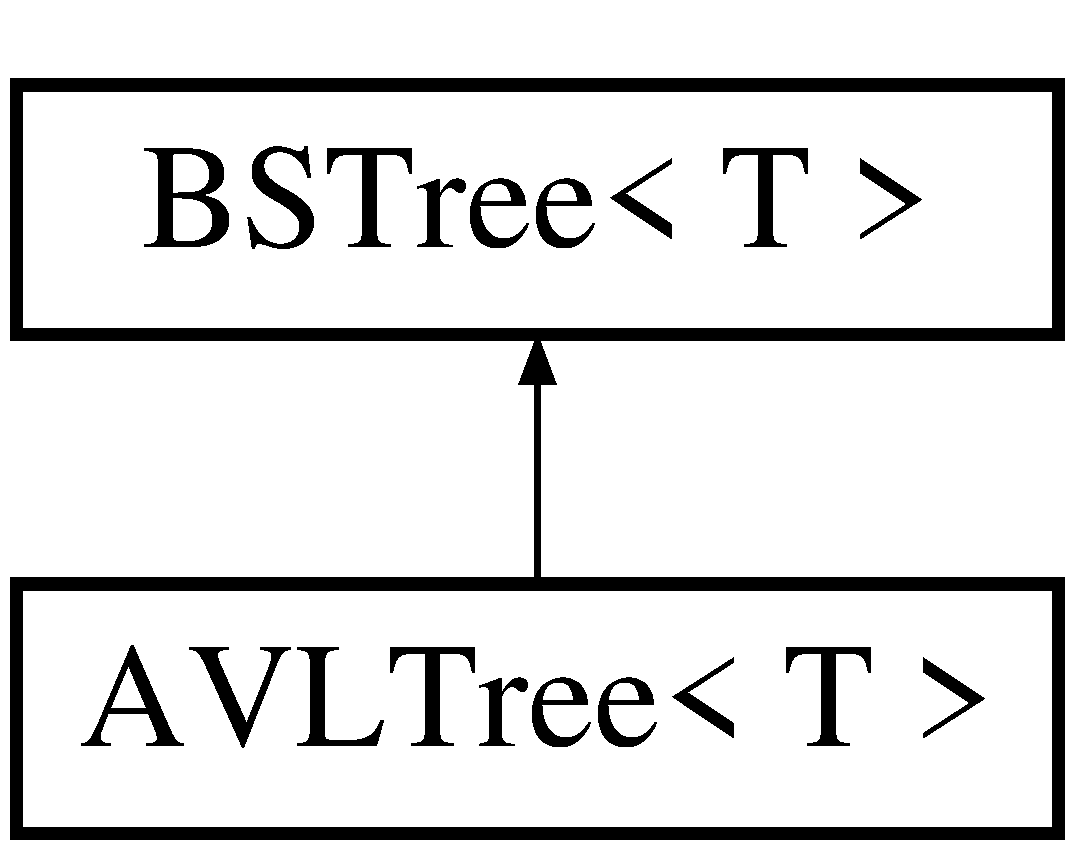
\includegraphics[height=2.000000cm]{classAVLTree}
\end{center}
\end{figure}
\subsection*{Public Types}
\begin{DoxyCompactItemize}
\item 
\hypertarget{classAVLTree_a384ae4f11fd0ceefeefd3670df15d478}{typedef \hyperlink{classBSTree}{B\-S\-Tree}$<$ T $>$\-::\hyperlink{structBSTree_1_1BinTreeNode}{Bin\-Tree\-Node} $\ast$ \hyperlink{classAVLTree_a384ae4f11fd0ceefeefd3670df15d478}{Bin\-Tree}}\label{classAVLTree_a384ae4f11fd0ceefeefd3670df15d478}

\begin{DoxyCompactList}\small\item\em making typename for compiler to resolve recognizing bintree$\ast$ \end{DoxyCompactList}\item 
\hypertarget{classAVLTree_a787ae799f7ceb9c9dc8d35b58207479b}{typedef std\-::stack$<$ \hyperlink{classBSTree_ae961195e523a45be64a981840e953b67}{Bin\-Tree} $>$ \hyperlink{classAVLTree_a787ae799f7ceb9c9dc8d35b58207479b}{stack}}\label{classAVLTree_a787ae799f7ceb9c9dc8d35b58207479b}

\begin{DoxyCompactList}\small\item\em defining type for transparency (mostly for myself) \end{DoxyCompactList}\end{DoxyCompactItemize}
\subsection*{Public Member Functions}
\begin{DoxyCompactItemize}
\item 
\hyperlink{classAVLTree_a8515cec8d90091c4b9e3d4feecc1f4f5}{A\-V\-L\-Tree} (Object\-Allocator $\ast$O\-A=0, bool Share\-O\-A=false)
\begin{DoxyCompactList}\small\item\em Constructor for \hyperlink{classAVLTree}{A\-V\-L\-Tree}. \end{DoxyCompactList}\item 
\hypertarget{classAVLTree_ae7bb44a235074a48d817acbc32846ae7}{virtual \hyperlink{classAVLTree_ae7bb44a235074a48d817acbc32846ae7}{$\sim$\-A\-V\-L\-Tree} ()}\label{classAVLTree_ae7bb44a235074a48d817acbc32846ae7}

\begin{DoxyCompactList}\small\item\em Destructor, will call base class destructor and that will be sufficient. \end{DoxyCompactList}\item 
virtual void \hyperlink{classAVLTree_ae389876cfbb5921623bed8111b921794}{insert} (const T \&value)
\begin{DoxyCompactList}\small\item\em Public insert function. Redirects to private recursive function to handle insertion. \end{DoxyCompactList}\item 
virtual void \hyperlink{classAVLTree_a53cda767b01115a3be8c1d839ef6d6c3}{remove} (const T \&value)
\begin{DoxyCompactList}\small\item\em Public remove function. Redirects to private recursive function. \end{DoxyCompactList}\end{DoxyCompactItemize}
\subsection*{Private Member Functions}
\begin{DoxyCompactItemize}
\item 
void \hyperlink{classAVLTree_ac19c4e70e093422cee80fc0ba3e22f4e}{Insert\-Item\-A\-V\-L} (\hyperlink{classBSTree_ae961195e523a45be64a981840e953b67}{Bin\-Tree} \&tree, const T \&value, \hyperlink{classAVLTree_a787ae799f7ceb9c9dc8d35b58207479b}{stack} \&nodes, int depth)
\begin{DoxyCompactList}\small\item\em Private recursive insert function to properly insert an item. \end{DoxyCompactList}\item 
void \hyperlink{classAVLTree_ad6178d2397e2ebbadacdbff42686e5dd}{Balance} (\hyperlink{classAVLTree_a787ae799f7ceb9c9dc8d35b58207479b}{stack} \&nodes, bool Inserting=true)
\begin{DoxyCompactList}\small\item\em Balances an A\-V\-L Tree. \end{DoxyCompactList}\item 
void \hyperlink{classAVLTree_a148755819d554e81505d952c7dd35f03}{Rotate\-Left} (\hyperlink{classBSTree_ae961195e523a45be64a981840e953b67}{Bin\-Tree} \&tree)
\begin{DoxyCompactList}\small\item\em Rotate a node left. \end{DoxyCompactList}\item 
void \hyperlink{classAVLTree_a111e0d371175d4c4c4e1560cfe8172b1}{Rotate\-Right} (\hyperlink{classBSTree_ae961195e523a45be64a981840e953b67}{Bin\-Tree} \&tree)
\begin{DoxyCompactList}\small\item\em Rotate a node right. \end{DoxyCompactList}\item 
void \hyperlink{classAVLTree_ad51f5fe9ab61c0d207c326c36b3a7cce}{Delete\-Item\-A\-V\-L} (\hyperlink{classBSTree_ae961195e523a45be64a981840e953b67}{Bin\-Tree} \&tree, const T \&value, std\-::stack$<$ \hyperlink{classBSTree_ae961195e523a45be64a981840e953b67}{Bin\-Tree} $>$ \&nodes)
\begin{DoxyCompactList}\small\item\em Deleting an item in avl tree. \end{DoxyCompactList}\item 
void \hyperlink{classAVLTree_a0ae4359dfca1abb5f18a7b4a3b80ebb8}{Attach\-Rotation} (\hyperlink{classBSTree_ae961195e523a45be64a981840e953b67}{Bin\-Tree} \&parent, \hyperlink{classBSTree_ae961195e523a45be64a981840e953b67}{Bin\-Tree} \&rotation)
\begin{DoxyCompactList}\small\item\em Reataches a rotation since we dont inheritanly have a parent pointer. \end{DoxyCompactList}\item 
void \hyperlink{classAVLTree_ac3f380ad5c5fd3175333a95adeba6174}{Left\-Heavy\-Balance} (\hyperlink{classBSTree_ae961195e523a45be64a981840e953b67}{Bin\-Tree} \&y, std\-::stack$<$ \hyperlink{classBSTree_ae961195e523a45be64a981840e953b67}{Bin\-Tree} $>$ \&nodes)
\begin{DoxyCompactList}\small\item\em Balance if offending node is left heavy. \end{DoxyCompactList}\item 
void \hyperlink{classAVLTree_abce0a7342b0663127c8ff9b633bb765f}{Right\-Heavy\-Balance} (\hyperlink{classBSTree_ae961195e523a45be64a981840e953b67}{Bin\-Tree} \&y, std\-::stack$<$ \hyperlink{classBSTree_ae961195e523a45be64a981840e953b67}{Bin\-Tree} $>$ \&nodes)
\begin{DoxyCompactList}\small\item\em Balance if we are right heavy. \end{DoxyCompactList}\end{DoxyCompactItemize}
\subsection*{Additional Inherited Members}


\subsection{Detailed Description}
\subsubsection*{template$<$typename T$>$class A\-V\-L\-Tree$<$ T $>$}

avl tree class 

\subsection{Constructor \& Destructor Documentation}
\hypertarget{classAVLTree_a8515cec8d90091c4b9e3d4feecc1f4f5}{\index{A\-V\-L\-Tree@{A\-V\-L\-Tree}!A\-V\-L\-Tree@{A\-V\-L\-Tree}}
\index{A\-V\-L\-Tree@{A\-V\-L\-Tree}!AVLTree@{A\-V\-L\-Tree}}
\subsubsection[{A\-V\-L\-Tree}]{\setlength{\rightskip}{0pt plus 5cm}template$<$typename T $>$ {\bf A\-V\-L\-Tree}$<$ T $>$\-::{\bf A\-V\-L\-Tree} (
\begin{DoxyParamCaption}
\item[{Object\-Allocator $\ast$}]{O\-A = {\ttfamily 0}, }
\item[{bool}]{Share\-O\-A = {\ttfamily false}}
\end{DoxyParamCaption}
)}}\label{classAVLTree_a8515cec8d90091c4b9e3d4feecc1f4f5}


Constructor for \hyperlink{classAVLTree}{A\-V\-L\-Tree}. 


\begin{DoxyParams}{Parameters}
{\em O\-A} & Object Allocator to be used with the tree. (either provided or object makes its own).\\
\hline
{\em Share\-O\-A} & Flag to indicate sharing of an allocator between copies of objects \\
\hline
\end{DoxyParams}


\subsection{Member Function Documentation}
\hypertarget{classAVLTree_a0ae4359dfca1abb5f18a7b4a3b80ebb8}{\index{A\-V\-L\-Tree@{A\-V\-L\-Tree}!Attach\-Rotation@{Attach\-Rotation}}
\index{Attach\-Rotation@{Attach\-Rotation}!AVLTree@{A\-V\-L\-Tree}}
\subsubsection[{Attach\-Rotation}]{\setlength{\rightskip}{0pt plus 5cm}template$<$typename T $>$ void {\bf A\-V\-L\-Tree}$<$ T $>$\-::Attach\-Rotation (
\begin{DoxyParamCaption}
\item[{{\bf Bin\-Tree} \&}]{parent, }
\item[{{\bf Bin\-Tree} \&}]{rotation}
\end{DoxyParamCaption}
)\hspace{0.3cm}{\ttfamily [private]}}}\label{classAVLTree_a0ae4359dfca1abb5f18a7b4a3b80ebb8}


Reataches a rotation since we dont inheritanly have a parent pointer. 


\begin{DoxyParams}{Parameters}
{\em parent} & Parent of the offending node that was rotated.\\
\hline
{\em rotation} & The 'top' node (see diagram a few lines above, w is the 'top') of a rotation to hook back up. \\
\hline
\end{DoxyParams}
\hypertarget{classAVLTree_ad6178d2397e2ebbadacdbff42686e5dd}{\index{A\-V\-L\-Tree@{A\-V\-L\-Tree}!Balance@{Balance}}
\index{Balance@{Balance}!AVLTree@{A\-V\-L\-Tree}}
\subsubsection[{Balance}]{\setlength{\rightskip}{0pt plus 5cm}template$<$typename T $>$ void {\bf A\-V\-L\-Tree}$<$ T $>$\-::Balance (
\begin{DoxyParamCaption}
\item[{{\bf stack} \&}]{nodes, }
\item[{bool}]{Inserting = {\ttfamily true}}
\end{DoxyParamCaption}
)\hspace{0.3cm}{\ttfamily [private]}}}\label{classAVLTree_ad6178d2397e2ebbadacdbff42686e5dd}


Balances an A\-V\-L Tree. 


\begin{DoxyParams}{Parameters}
{\em nodes} & stack of where we went for insertion/deletion\\
\hline
{\em Inserting} & Bool to indicate whether we are balancing because of an insertion or deletion. If inserting we only need one rotation to fix the balance, if deleting we have to back track all the way up the tree. \\
\hline
\end{DoxyParams}
\hypertarget{classAVLTree_ad51f5fe9ab61c0d207c326c36b3a7cce}{\index{A\-V\-L\-Tree@{A\-V\-L\-Tree}!Delete\-Item\-A\-V\-L@{Delete\-Item\-A\-V\-L}}
\index{Delete\-Item\-A\-V\-L@{Delete\-Item\-A\-V\-L}!AVLTree@{A\-V\-L\-Tree}}
\subsubsection[{Delete\-Item\-A\-V\-L}]{\setlength{\rightskip}{0pt plus 5cm}template$<$typename T $>$ void {\bf A\-V\-L\-Tree}$<$ T $>$\-::Delete\-Item\-A\-V\-L (
\begin{DoxyParamCaption}
\item[{{\bf Bin\-Tree} \&}]{tree, }
\item[{const T \&}]{value, }
\item[{std\-::stack$<$ {\bf Bin\-Tree} $>$ \&}]{nodes}
\end{DoxyParamCaption}
)\hspace{0.3cm}{\ttfamily [private]}}}\label{classAVLTree_ad51f5fe9ab61c0d207c326c36b3a7cce}


Deleting an item in avl tree. 


\begin{DoxyParams}{Parameters}
{\em tree} & node to start at (in first call it is the root).\\
\hline
{\em value} & Value being removed from the tree\\
\hline
{\em nodes} & Stack of nodes we traversed to balance the tree after deletion \\
\hline
\end{DoxyParams}
\hypertarget{classAVLTree_ae389876cfbb5921623bed8111b921794}{\index{A\-V\-L\-Tree@{A\-V\-L\-Tree}!insert@{insert}}
\index{insert@{insert}!AVLTree@{A\-V\-L\-Tree}}
\subsubsection[{insert}]{\setlength{\rightskip}{0pt plus 5cm}template$<$typename T $>$ void {\bf A\-V\-L\-Tree}$<$ T $>$\-::insert (
\begin{DoxyParamCaption}
\item[{const T \&}]{value}
\end{DoxyParamCaption}
)\hspace{0.3cm}{\ttfamily [virtual]}}}\label{classAVLTree_ae389876cfbb5921623bed8111b921794}


Public insert function. Redirects to private recursive function to handle insertion. 


\begin{DoxyParams}{Parameters}
{\em value} & Whate is being inserted into the tree \\
\hline
\end{DoxyParams}


Reimplemented from \hyperlink{classBSTree_aa7fc7600f30d0ecc0a75b25e11f6cc57}{B\-S\-Tree$<$ T $>$}.

\hypertarget{classAVLTree_ac19c4e70e093422cee80fc0ba3e22f4e}{\index{A\-V\-L\-Tree@{A\-V\-L\-Tree}!Insert\-Item\-A\-V\-L@{Insert\-Item\-A\-V\-L}}
\index{Insert\-Item\-A\-V\-L@{Insert\-Item\-A\-V\-L}!AVLTree@{A\-V\-L\-Tree}}
\subsubsection[{Insert\-Item\-A\-V\-L}]{\setlength{\rightskip}{0pt plus 5cm}template$<$typename T $>$ void {\bf A\-V\-L\-Tree}$<$ T $>$\-::Insert\-Item\-A\-V\-L (
\begin{DoxyParamCaption}
\item[{{\bf Bin\-Tree} \&}]{tree, }
\item[{const T \&}]{value, }
\item[{{\bf stack} \&}]{nodes, }
\item[{int}]{depth}
\end{DoxyParamCaption}
)\hspace{0.3cm}{\ttfamily [private]}}}\label{classAVLTree_ac19c4e70e093422cee80fc0ba3e22f4e}


Private recursive insert function to properly insert an item. 


\begin{DoxyParams}{Parameters}
{\em tree} & Reference to a pointer of the root of the tree\\
\hline
{\em value} & What's being added to the tree\\
\hline
{\em nodes} & Reference to a stack to keep track of where we went to balance the tree after inserting.\\
\hline
{\em depth} & How deep down the tree we went. Used to update height \\
\hline
\end{DoxyParams}
\hypertarget{classAVLTree_ac3f380ad5c5fd3175333a95adeba6174}{\index{A\-V\-L\-Tree@{A\-V\-L\-Tree}!Left\-Heavy\-Balance@{Left\-Heavy\-Balance}}
\index{Left\-Heavy\-Balance@{Left\-Heavy\-Balance}!AVLTree@{A\-V\-L\-Tree}}
\subsubsection[{Left\-Heavy\-Balance}]{\setlength{\rightskip}{0pt plus 5cm}template$<$typename T $>$ void {\bf A\-V\-L\-Tree}$<$ T $>$\-::Left\-Heavy\-Balance (
\begin{DoxyParamCaption}
\item[{{\bf Bin\-Tree} \&}]{y, }
\item[{std\-::stack$<$ {\bf Bin\-Tree} $>$ \&}]{nodes}
\end{DoxyParamCaption}
)\hspace{0.3cm}{\ttfamily [private]}}}\label{classAVLTree_ac3f380ad5c5fd3175333a95adeba6174}


Balance if offending node is left heavy. 


\begin{DoxyParams}{Parameters}
{\em y} & Offending node\\
\hline
{\em nodes} & stack of nodes traveled. needed to get parent of y to rotate \\
\hline
\end{DoxyParams}
\hypertarget{classAVLTree_a53cda767b01115a3be8c1d839ef6d6c3}{\index{A\-V\-L\-Tree@{A\-V\-L\-Tree}!remove@{remove}}
\index{remove@{remove}!AVLTree@{A\-V\-L\-Tree}}
\subsubsection[{remove}]{\setlength{\rightskip}{0pt plus 5cm}template$<$typename T $>$ void {\bf A\-V\-L\-Tree}$<$ T $>$\-::remove (
\begin{DoxyParamCaption}
\item[{const T \&}]{value}
\end{DoxyParamCaption}
)\hspace{0.3cm}{\ttfamily [virtual]}}}\label{classAVLTree_a53cda767b01115a3be8c1d839ef6d6c3}


Public remove function. Redirects to private recursive function. 


\begin{DoxyParams}{Parameters}
{\em value} & What's being removed from the tree. \\
\hline
\end{DoxyParams}


Reimplemented from \hyperlink{classBSTree_a6b930b09010b674ca6b09c88bd3effeb}{B\-S\-Tree$<$ T $>$}.

\hypertarget{classAVLTree_abce0a7342b0663127c8ff9b633bb765f}{\index{A\-V\-L\-Tree@{A\-V\-L\-Tree}!Right\-Heavy\-Balance@{Right\-Heavy\-Balance}}
\index{Right\-Heavy\-Balance@{Right\-Heavy\-Balance}!AVLTree@{A\-V\-L\-Tree}}
\subsubsection[{Right\-Heavy\-Balance}]{\setlength{\rightskip}{0pt plus 5cm}template$<$typename T $>$ void {\bf A\-V\-L\-Tree}$<$ T $>$\-::Right\-Heavy\-Balance (
\begin{DoxyParamCaption}
\item[{{\bf Bin\-Tree} \&}]{y, }
\item[{std\-::stack$<$ {\bf Bin\-Tree} $>$ \&}]{nodes}
\end{DoxyParamCaption}
)\hspace{0.3cm}{\ttfamily [private]}}}\label{classAVLTree_abce0a7342b0663127c8ff9b633bb765f}


Balance if we are right heavy. 


\begin{DoxyParams}{Parameters}
{\em y} & The node that is out of balance.\\
\hline
{\em nodes} & Stack of nodes we traveled. Need to get the parent of y to properly rotate. \\
\hline
\end{DoxyParams}
\hypertarget{classAVLTree_a148755819d554e81505d952c7dd35f03}{\index{A\-V\-L\-Tree@{A\-V\-L\-Tree}!Rotate\-Left@{Rotate\-Left}}
\index{Rotate\-Left@{Rotate\-Left}!AVLTree@{A\-V\-L\-Tree}}
\subsubsection[{Rotate\-Left}]{\setlength{\rightskip}{0pt plus 5cm}template$<$typename T $>$ void {\bf A\-V\-L\-Tree}$<$ T $>$\-::Rotate\-Left (
\begin{DoxyParamCaption}
\item[{{\bf Bin\-Tree} \&}]{tree}
\end{DoxyParamCaption}
)\hspace{0.3cm}{\ttfamily [private]}}}\label{classAVLTree_a148755819d554e81505d952c7dd35f03}


Rotate a node left. 


\begin{DoxyParams}{Parameters}
{\em tree} & Offending node \\
\hline
\end{DoxyParams}
\hypertarget{classAVLTree_a111e0d371175d4c4c4e1560cfe8172b1}{\index{A\-V\-L\-Tree@{A\-V\-L\-Tree}!Rotate\-Right@{Rotate\-Right}}
\index{Rotate\-Right@{Rotate\-Right}!AVLTree@{A\-V\-L\-Tree}}
\subsubsection[{Rotate\-Right}]{\setlength{\rightskip}{0pt plus 5cm}template$<$typename T $>$ void {\bf A\-V\-L\-Tree}$<$ T $>$\-::Rotate\-Right (
\begin{DoxyParamCaption}
\item[{{\bf Bin\-Tree} \&}]{tree}
\end{DoxyParamCaption}
)\hspace{0.3cm}{\ttfamily [private]}}}\label{classAVLTree_a111e0d371175d4c4c4e1560cfe8172b1}


Rotate a node right. 


\begin{DoxyParams}{Parameters}
{\em tree} & the offending node \\
\hline
\end{DoxyParams}


The documentation for this class was generated from the following files\-:\begin{DoxyCompactItemize}
\item 
\hyperlink{AVLTree_8h}{A\-V\-L\-Tree.\-h}\item 
\hyperlink{AVLTree_8cpp}{A\-V\-L\-Tree.\-cpp}\end{DoxyCompactItemize}

\hypertarget{structBSTree_1_1BinTreeNode}{\section{B\-S\-Tree$<$ T $>$\-:\-:Bin\-Tree\-Node Struct Reference}
\label{structBSTree_1_1BinTreeNode}\index{B\-S\-Tree$<$ T $>$\-::\-Bin\-Tree\-Node@{B\-S\-Tree$<$ T $>$\-::\-Bin\-Tree\-Node}}
}


node class used in the binary tree  




{\ttfamily \#include $<$B\-S\-Tree.\-h$>$}

\subsection*{Public Member Functions}
\begin{DoxyCompactItemize}
\item 
\hypertarget{structBSTree_1_1BinTreeNode_ae3214dd7d735bf71c9e05d8e55613390}{\hyperlink{structBSTree_1_1BinTreeNode_ae3214dd7d735bf71c9e05d8e55613390}{Bin\-Tree\-Node} (const T \&value)}\label{structBSTree_1_1BinTreeNode_ae3214dd7d735bf71c9e05d8e55613390}

\begin{DoxyCompactList}\small\item\em constructor for the nodes \end{DoxyCompactList}\end{DoxyCompactItemize}
\subsection*{Public Attributes}
\begin{DoxyCompactItemize}
\item 
\hypertarget{structBSTree_1_1BinTreeNode_af22176f541cb6df427f0b9e4412ba4e9}{\hyperlink{structBSTree_1_1BinTreeNode}{Bin\-Tree\-Node} $\ast$ \hyperlink{structBSTree_1_1BinTreeNode_af22176f541cb6df427f0b9e4412ba4e9}{left}}\label{structBSTree_1_1BinTreeNode_af22176f541cb6df427f0b9e4412ba4e9}

\begin{DoxyCompactList}\small\item\em pointer to left child \end{DoxyCompactList}\item 
\hypertarget{structBSTree_1_1BinTreeNode_a8c7c02ca8cabae3a9bbb1958b19447e1}{\hyperlink{structBSTree_1_1BinTreeNode}{Bin\-Tree\-Node} $\ast$ \hyperlink{structBSTree_1_1BinTreeNode_a8c7c02ca8cabae3a9bbb1958b19447e1}{right}}\label{structBSTree_1_1BinTreeNode_a8c7c02ca8cabae3a9bbb1958b19447e1}

\begin{DoxyCompactList}\small\item\em pointer to right child \end{DoxyCompactList}\item 
\hypertarget{structBSTree_1_1BinTreeNode_a8d9d139d8c90693026b394683653eeb1}{T \hyperlink{structBSTree_1_1BinTreeNode_a8d9d139d8c90693026b394683653eeb1}{data}}\label{structBSTree_1_1BinTreeNode_a8d9d139d8c90693026b394683653eeb1}

\begin{DoxyCompactList}\small\item\em information in the ndoe \end{DoxyCompactList}\item 
\hypertarget{structBSTree_1_1BinTreeNode_a24e8cb513683763ada843e903e427a6a}{int \hyperlink{structBSTree_1_1BinTreeNode_a24e8cb513683763ada843e903e427a6a}{balance\-\_\-factor}}\label{structBSTree_1_1BinTreeNode_a24e8cb513683763ada843e903e427a6a}

\begin{DoxyCompactList}\small\item\em optional(not implemeneted) \end{DoxyCompactList}\item 
\hypertarget{structBSTree_1_1BinTreeNode_a682c20cabecc4bffc0f0d98d870a7490}{unsigned \hyperlink{structBSTree_1_1BinTreeNode_a682c20cabecc4bffc0f0d98d870a7490}{count}}\label{structBSTree_1_1BinTreeNode_a682c20cabecc4bffc0f0d98d870a7490}

\begin{DoxyCompactList}\small\item\em number of nodes in subtree(not used) \end{DoxyCompactList}\end{DoxyCompactItemize}


\subsection{Detailed Description}
\subsubsection*{template$<$typename T$>$struct B\-S\-Tree$<$ T $>$\-::\-Bin\-Tree\-Node}

node class used in the binary tree 

The documentation for this struct was generated from the following file\-:\begin{DoxyCompactItemize}
\item 
\hyperlink{BSTree_8h}{B\-S\-Tree.\-h}\end{DoxyCompactItemize}

\hypertarget{classBSTException}{\section{B\-S\-T\-Exception Class Reference}
\label{classBSTException}\index{B\-S\-T\-Exception@{B\-S\-T\-Exception}}
}


exception class  




{\ttfamily \#include $<$B\-S\-Tree.\-h$>$}

Inheritance diagram for B\-S\-T\-Exception\-:\begin{figure}[H]
\begin{center}
\leavevmode
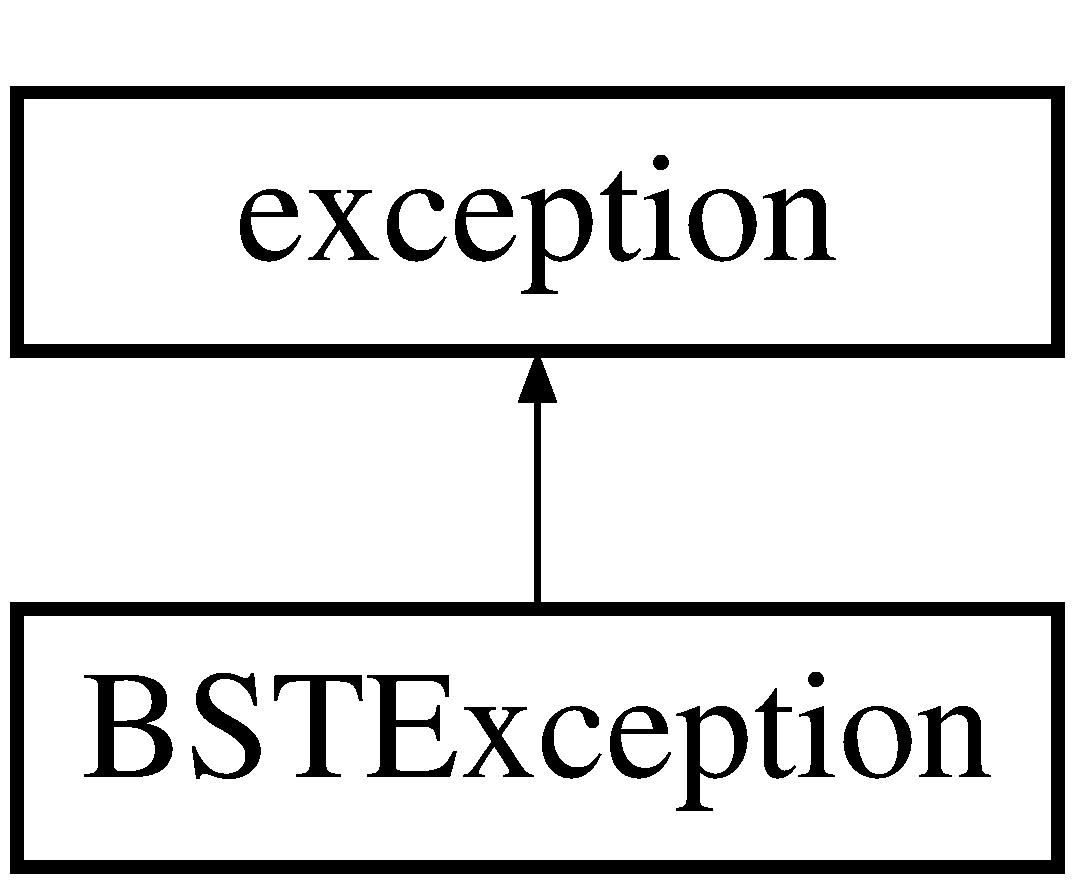
\includegraphics[height=2.000000cm]{classBSTException}
\end{center}
\end{figure}
\subsection*{Public Types}
\begin{DoxyCompactItemize}
\item 
enum \hyperlink{classBSTException_a4fffb763ca6b98d6b1329d546e76d8d8}{B\-S\-T\-\_\-\-E\-X\-C\-E\-P\-T\-I\-O\-N} \{ {\bfseries E\-\_\-\-D\-U\-P\-L\-I\-C\-A\-T\-E}, 
{\bfseries E\-\_\-\-N\-O\-\_\-\-M\-E\-M\-O\-R\-Y}
 \}
\begin{DoxyCompactList}\small\item\em error type for exceptions \end{DoxyCompactList}\end{DoxyCompactItemize}
\subsection*{Public Member Functions}
\begin{DoxyCompactItemize}
\item 
\hypertarget{classBSTException_af7683167b01f3b0bcc1fa583aceedf7d}{\hyperlink{classBSTException_af7683167b01f3b0bcc1fa583aceedf7d}{B\-S\-T\-Exception} (int Err\-Code, const std\-::string \&Message)}\label{classBSTException_af7683167b01f3b0bcc1fa583aceedf7d}

\begin{DoxyCompactList}\small\item\em constructo for exception class \end{DoxyCompactList}\item 
\hypertarget{classBSTException_a7eb896dd6c636f528c7e0cf9fd203f97}{virtual int \hyperlink{classBSTException_a7eb896dd6c636f528c7e0cf9fd203f97}{code} (void) const }\label{classBSTException_a7eb896dd6c636f528c7e0cf9fd203f97}

\begin{DoxyCompactList}\small\item\em getter function to determine type of exception \end{DoxyCompactList}\item 
\hypertarget{classBSTException_a6dbecababd6976f8b3c880c8e422b1ca}{virtual const char $\ast$ \hyperlink{classBSTException_a6dbecababd6976f8b3c880c8e422b1ca}{what} (void) const   throw ()}\label{classBSTException_a6dbecababd6976f8b3c880c8e422b1ca}

\begin{DoxyCompactList}\small\item\em getter function to read message in exception \end{DoxyCompactList}\end{DoxyCompactItemize}
\subsection*{Private Attributes}
\begin{DoxyCompactItemize}
\item 
\hypertarget{classBSTException_a8fc812efe0dcfdc60448493b42e96d51}{int \hyperlink{classBSTException_a8fc812efe0dcfdc60448493b42e96d51}{error\-\_\-code\-\_\-}}\label{classBSTException_a8fc812efe0dcfdc60448493b42e96d51}

\begin{DoxyCompactList}\small\item\em type of exception \end{DoxyCompactList}\item 
\hypertarget{classBSTException_a94eb46d7c60fb2db7fa3ec8faf6e76c2}{std\-::string \hyperlink{classBSTException_a94eb46d7c60fb2db7fa3ec8faf6e76c2}{message\-\_\-}}\label{classBSTException_a94eb46d7c60fb2db7fa3ec8faf6e76c2}

\begin{DoxyCompactList}\small\item\em message for the exception \end{DoxyCompactList}\end{DoxyCompactItemize}


\subsection{Detailed Description}
exception class 

The documentation for this class was generated from the following file\-:\begin{DoxyCompactItemize}
\item 
\hyperlink{BSTree_8h}{B\-S\-Tree.\-h}\end{DoxyCompactItemize}

\hypertarget{classBSTree}{\section{B\-S\-Tree$<$ T $>$ Class Template Reference}
\label{classBSTree}\index{B\-S\-Tree$<$ T $>$@{B\-S\-Tree$<$ T $>$}}
}


binary search tree class  




{\ttfamily \#include $<$B\-S\-Tree.\-h$>$}

Inheritance diagram for B\-S\-Tree$<$ T $>$\-:\begin{figure}[H]
\begin{center}
\leavevmode
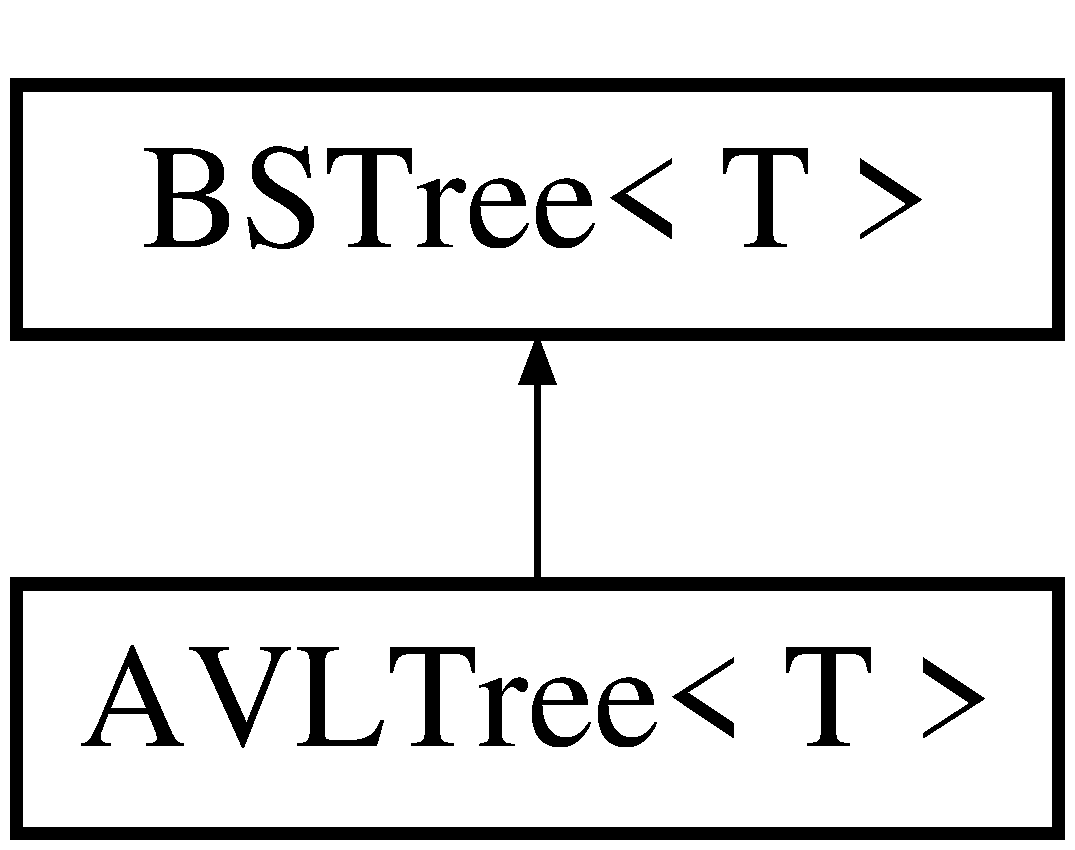
\includegraphics[height=2.000000cm]{classBSTree}
\end{center}
\end{figure}
\subsection*{Classes}
\begin{DoxyCompactItemize}
\item 
struct \hyperlink{structBSTree_1_1BinTreeNode}{Bin\-Tree\-Node}
\begin{DoxyCompactList}\small\item\em node class used in the binary tree \end{DoxyCompactList}\end{DoxyCompactItemize}
\subsection*{Public Types}
\begin{DoxyCompactItemize}
\item 
\hypertarget{classBSTree_ae961195e523a45be64a981840e953b67}{typedef \hyperlink{structBSTree_1_1BinTreeNode}{Bin\-Tree\-Node} $\ast$ \hyperlink{classBSTree_ae961195e523a45be64a981840e953b67}{Bin\-Tree}}\label{classBSTree_ae961195e523a45be64a981840e953b67}

\begin{DoxyCompactList}\small\item\em simplification for ease of use \end{DoxyCompactList}\end{DoxyCompactItemize}
\subsection*{Public Member Functions}
\begin{DoxyCompactItemize}
\item 
\hyperlink{classBSTree_ab5ad17b82195c7758ebbb9b6f41229e6}{B\-S\-Tree} (Object\-Allocator $\ast$O\-A=0, bool Share\-O\-A=false)
\begin{DoxyCompactList}\small\item\em Constructor for B\-S\-T. \end{DoxyCompactList}\item 
\hyperlink{classBSTree_ac05b0777b5942ea93fe292cbe4c67059}{B\-S\-Tree} (const \hyperlink{classBSTree}{B\-S\-Tree} \&rhs)
\begin{DoxyCompactList}\small\item\em Copy constructor. \end{DoxyCompactList}\item 
\hypertarget{classBSTree_a9e318eddca027a4ca500e6b7c84c749f}{virtual \hyperlink{classBSTree_a9e318eddca027a4ca500e6b7c84c749f}{$\sim$\-B\-S\-Tree} ()}\label{classBSTree_a9e318eddca027a4ca500e6b7c84c749f}

\begin{DoxyCompactList}\small\item\em Destructor. \end{DoxyCompactList}\item 
\hyperlink{classBSTree}{B\-S\-Tree}$<$ T $>$ \& \hyperlink{classBSTree_a7f20b5a0e6a3114b402085b00b7878ab}{operator=} (const \hyperlink{classBSTree}{B\-S\-Tree} \&rhs)
\begin{DoxyCompactList}\small\item\em Assignment operator. \end{DoxyCompactList}\item 
const \hyperlink{structBSTree_1_1BinTreeNode}{Bin\-Tree\-Node} $\ast$ \hyperlink{classBSTree_ad0369e593a64399537242a6ee3656a69}{operator\mbox{[}$\,$\mbox{]}} (int index) const 
\begin{DoxyCompactList}\small\item\em Indexing operator (not implemented). \end{DoxyCompactList}\item 
virtual void \hyperlink{classBSTree_aa7fc7600f30d0ecc0a75b25e11f6cc57}{insert} (const T \&value)
\begin{DoxyCompactList}\small\item\em Public insert function. Redirects to private recursive function to handle insertion. \end{DoxyCompactList}\item 
virtual void \hyperlink{classBSTree_a6b930b09010b674ca6b09c88bd3effeb}{remove} (const T \&value)
\begin{DoxyCompactList}\small\item\em Public removal function. Redirects to private recursive function. \end{DoxyCompactList}\item 
\hypertarget{classBSTree_ab4ec7dcce20e9bf8a3e09b371d3af73d}{void \hyperlink{classBSTree_ab4ec7dcce20e9bf8a3e09b371d3af73d}{clear} (void)}\label{classBSTree_ab4ec7dcce20e9bf8a3e09b371d3af73d}

\begin{DoxyCompactList}\small\item\em Removes all nodes from the tree. Calls recursive function. \end{DoxyCompactList}\item 
bool \hyperlink{classBSTree_a4c789a7e91d8a21074ae6ed6be42ac4a}{find} (const T \&value, unsigned \&compares) const 
\begin{DoxyCompactList}\small\item\em Finds an item in the tree. Calls recursive function to do the work. \end{DoxyCompactList}\item 
bool \hyperlink{classBSTree_aef431a55bc9069dcd17c15b4ddacf48e}{empty} (void) const 
\begin{DoxyCompactList}\small\item\em Checks if the tree is empty. \end{DoxyCompactList}\item 
unsigned int \hyperlink{classBSTree_acaf31244510bb689f8bf1cf83fb4b212}{size} (void) const 
\begin{DoxyCompactList}\small\item\em Returns number of nodes in the tree. \end{DoxyCompactList}\item 
int \hyperlink{classBSTree_a4f2b0cd077e99415954cf1162c282306}{height} (void) const 
\begin{DoxyCompactList}\small\item\em Checks height of the tree. \end{DoxyCompactList}\item 
\hyperlink{classBSTree_ae961195e523a45be64a981840e953b67}{Bin\-Tree} \hyperlink{classBSTree_a84c029bf53eb4e50b4d14f610a46ef2a}{root} (void) const 
\begin{DoxyCompactList}\small\item\em Returns root of the tree. \end{DoxyCompactList}\end{DoxyCompactItemize}
\subsection*{Static Public Member Functions}
\begin{DoxyCompactItemize}
\item 
static bool \hyperlink{classBSTree_afed4448d4cf9b7cf36bf0efb79405931}{Implemented\-Indexing} (void)
\begin{DoxyCompactList}\small\item\em Checks for extra credit implementation. \end{DoxyCompactList}\end{DoxyCompactItemize}
\subsection*{Protected Member Functions}
\begin{DoxyCompactItemize}
\item 
\hyperlink{classBSTree_ae961195e523a45be64a981840e953b67}{Bin\-Tree} \hyperlink{classBSTree_a246963de859d3fc8cb7c9d5a2c2bf87f}{make\-\_\-node} (const T \&value)
\begin{DoxyCompactList}\small\item\em Makes a node to put in the tree. \end{DoxyCompactList}\item 
void \hyperlink{classBSTree_ad1c3dedcd1d2172d767058a5afc48700}{Free\-Node} (\hyperlink{classBSTree_ae961195e523a45be64a981840e953b67}{Bin\-Tree} node)
\begin{DoxyCompactList}\small\item\em First deleted underlying node in the allocator and then gives back thta memory to the allocator. \end{DoxyCompactList}\item 
int \hyperlink{classBSTree_aaa3acfb629509ec0797c149e0307b59e}{tree\-\_\-height} (\hyperlink{classBSTree_ae961195e523a45be64a981840e953b67}{Bin\-Tree} tree) const 
\begin{DoxyCompactList}\small\item\em Calculate height of the tree. \end{DoxyCompactList}\item 
void \hyperlink{classBSTree_a7c864388c9ce422b7329e7561c30a316}{Find\-Predecessor} (\hyperlink{classBSTree_ae961195e523a45be64a981840e953b67}{Bin\-Tree} tree, \hyperlink{classBSTree_ae961195e523a45be64a981840e953b67}{Bin\-Tree} \&predecessor) const 
\begin{DoxyCompactList}\small\item\em Finds predecessor of a node. \end{DoxyCompactList}\item 
void \hyperlink{classBSTree_a9aee3782f0daf87e0e2ec1f3aedb4f5e}{Clear\-Rec} (\hyperlink{classBSTree_ae961195e523a45be64a981840e953b67}{Bin\-Tree} tree)
\begin{DoxyCompactList}\small\item\em removes all nodes in the tree \end{DoxyCompactList}\item 
virtual void \hyperlink{classBSTree_aa32cf54d2ea8cfc413293d0538446aad}{Insert\-Item} (\hyperlink{classBSTree_ae961195e523a45be64a981840e953b67}{Bin\-Tree} \&tree, const T \&value, int depth)
\begin{DoxyCompactList}\small\item\em Recursively inserts an item into the tree. \end{DoxyCompactList}\end{DoxyCompactItemize}
\subsection*{Protected Attributes}
\begin{DoxyCompactItemize}
\item 
\hypertarget{classBSTree_acbccf64f8c26330090cbc5d8d9001195}{\hyperlink{classBSTree_ae961195e523a45be64a981840e953b67}{Bin\-Tree} \hyperlink{classBSTree_acbccf64f8c26330090cbc5d8d9001195}{Root}}\label{classBSTree_acbccf64f8c26330090cbc5d8d9001195}

\begin{DoxyCompactList}\small\item\em the head of the tree \end{DoxyCompactList}\item 
\hypertarget{classBSTree_a5e6cde514ed0ba271e1c017ed402b1f9}{Object\-Allocator $\ast$ \hyperlink{classBSTree_a5e6cde514ed0ba271e1c017ed402b1f9}{allocator}}\label{classBSTree_a5e6cde514ed0ba271e1c017ed402b1f9}

\begin{DoxyCompactList}\small\item\em pointer to object allocator \end{DoxyCompactList}\item 
\hypertarget{classBSTree_a427ba240384aabc139b442e1c8b6125c}{int \hyperlink{classBSTree_a427ba240384aabc139b442e1c8b6125c}{Height}}\label{classBSTree_a427ba240384aabc139b442e1c8b6125c}

\begin{DoxyCompactList}\small\item\em height of the tree \end{DoxyCompactList}\item 
\hypertarget{classBSTree_ae77fc08bcf3775741578e616d8f98b66}{unsigned int \hyperlink{classBSTree_ae77fc08bcf3775741578e616d8f98b66}{Num\-Nodes}}\label{classBSTree_ae77fc08bcf3775741578e616d8f98b66}

\begin{DoxyCompactList}\small\item\em number of nodes in the tree \end{DoxyCompactList}\item 
bool \hyperlink{classBSTree_afcb0096e560f0d4a7a44c23bf17883f1}{Own\-O\-A}
\item 
bool \hyperlink{classBSTree_aa93a52c804477d1683cc2197da61bc1f}{Share\-Alloc}
\end{DoxyCompactItemize}
\subsection*{Private Member Functions}
\begin{DoxyCompactItemize}
\item 
void \hyperlink{classBSTree_ab62ef6fa7acb74aefd5177977aeb4636}{Copy\-Helper} (\hyperlink{classBSTree_ae961195e523a45be64a981840e953b67}{Bin\-Tree} \&destination, const \hyperlink{classBSTree_ae961195e523a45be64a981840e953b67}{Bin\-Tree} \&source)
\begin{DoxyCompactList}\small\item\em Recursive copy function used in copy construcotr and assignment. \end{DoxyCompactList}\item 
virtual void \hyperlink{classBSTree_acce425c45a5c61fd887627740d123d0d}{Delete\-Item} (\hyperlink{classBSTree_ae961195e523a45be64a981840e953b67}{Bin\-Tree} \&tree, const T \&Data)
\begin{DoxyCompactList}\small\item\em Recursive function to remove an item from the tree. \end{DoxyCompactList}\item 
bool \hyperlink{classBSTree_a2ff8b3553c3ae8f6aeadab1598ca22d3}{Find\-Item} (\hyperlink{classBSTree_ae961195e523a45be64a981840e953b67}{Bin\-Tree} tree, const T \&Data, unsigned \&compares) const 
\begin{DoxyCompactList}\small\item\em Finds an item in the tree. \end{DoxyCompactList}\end{DoxyCompactItemize}


\subsection{Detailed Description}
\subsubsection*{template$<$typename T$>$class B\-S\-Tree$<$ T $>$}

binary search tree class 

\subsection{Constructor \& Destructor Documentation}
\hypertarget{classBSTree_ab5ad17b82195c7758ebbb9b6f41229e6}{\index{B\-S\-Tree@{B\-S\-Tree}!B\-S\-Tree@{B\-S\-Tree}}
\index{B\-S\-Tree@{B\-S\-Tree}!BSTree@{B\-S\-Tree}}
\subsubsection[{B\-S\-Tree}]{\setlength{\rightskip}{0pt plus 5cm}template$<$typename T $>$ {\bf B\-S\-Tree}$<$ T $>$\-::{\bf B\-S\-Tree} (
\begin{DoxyParamCaption}
\item[{Object\-Allocator $\ast$}]{O\-A = {\ttfamily 0}, }
\item[{bool}]{Share\-O\-A = {\ttfamily false}}
\end{DoxyParamCaption}
)}}\label{classBSTree_ab5ad17b82195c7758ebbb9b6f41229e6}


Constructor for B\-S\-T. 


\begin{DoxyParams}{Parameters}
{\em O\-A} & Object\-Allocator to use with the tree (either provided or created).\\
\hline
{\em Share\-O\-A} & Flag to indicate sharing of the object allocator with copies of the object. \\
\hline
\end{DoxyParams}
\hypertarget{classBSTree_ac05b0777b5942ea93fe292cbe4c67059}{\index{B\-S\-Tree@{B\-S\-Tree}!B\-S\-Tree@{B\-S\-Tree}}
\index{B\-S\-Tree@{B\-S\-Tree}!BSTree@{B\-S\-Tree}}
\subsubsection[{B\-S\-Tree}]{\setlength{\rightskip}{0pt plus 5cm}template$<$typename T $>$ {\bf B\-S\-Tree}$<$ T $>$\-::{\bf B\-S\-Tree} (
\begin{DoxyParamCaption}
\item[{const {\bf B\-S\-Tree}$<$ T $>$ \&}]{rhs}
\end{DoxyParamCaption}
)}}\label{classBSTree_ac05b0777b5942ea93fe292cbe4c67059}


Copy constructor. 


\begin{DoxyParams}{Parameters}
{\em rhs} & Object being copied \\
\hline
\end{DoxyParams}


\subsection{Member Function Documentation}
\hypertarget{classBSTree_a9aee3782f0daf87e0e2ec1f3aedb4f5e}{\index{B\-S\-Tree@{B\-S\-Tree}!Clear\-Rec@{Clear\-Rec}}
\index{Clear\-Rec@{Clear\-Rec}!BSTree@{B\-S\-Tree}}
\subsubsection[{Clear\-Rec}]{\setlength{\rightskip}{0pt plus 5cm}template$<$typename T $>$ void {\bf B\-S\-Tree}$<$ T $>$\-::Clear\-Rec (
\begin{DoxyParamCaption}
\item[{{\bf Bin\-Tree}}]{tree}
\end{DoxyParamCaption}
)\hspace{0.3cm}{\ttfamily [protected]}}}\label{classBSTree_a9aee3782f0daf87e0e2ec1f3aedb4f5e}


removes all nodes in the tree 

Recursive functio to delete all nodes in the tree.


\begin{DoxyParams}{Parameters}
{\em tree} & node being removed \\
\hline
\end{DoxyParams}
\hypertarget{classBSTree_ab62ef6fa7acb74aefd5177977aeb4636}{\index{B\-S\-Tree@{B\-S\-Tree}!Copy\-Helper@{Copy\-Helper}}
\index{Copy\-Helper@{Copy\-Helper}!BSTree@{B\-S\-Tree}}
\subsubsection[{Copy\-Helper}]{\setlength{\rightskip}{0pt plus 5cm}template$<$typename T $>$ void {\bf B\-S\-Tree}$<$ T $>$\-::Copy\-Helper (
\begin{DoxyParamCaption}
\item[{{\bf Bin\-Tree} \&}]{destination, }
\item[{const {\bf Bin\-Tree} \&}]{source}
\end{DoxyParamCaption}
)\hspace{0.3cm}{\ttfamily [private]}}}\label{classBSTree_ab62ef6fa7acb74aefd5177977aeb4636}


Recursive copy function used in copy construcotr and assignment. 


\begin{DoxyParams}{Parameters}
{\em destination} & lhs object\\
\hline
{\em source} & rhs object \\
\hline
\end{DoxyParams}
\hypertarget{classBSTree_acce425c45a5c61fd887627740d123d0d}{\index{B\-S\-Tree@{B\-S\-Tree}!Delete\-Item@{Delete\-Item}}
\index{Delete\-Item@{Delete\-Item}!BSTree@{B\-S\-Tree}}
\subsubsection[{Delete\-Item}]{\setlength{\rightskip}{0pt plus 5cm}template$<$typename T$>$ void {\bf B\-S\-Tree}$<$ T $>$\-::Delete\-Item (
\begin{DoxyParamCaption}
\item[{{\bf Bin\-Tree} \&}]{tree, }
\item[{const T \&}]{Data}
\end{DoxyParamCaption}
)\hspace{0.3cm}{\ttfamily [private]}, {\ttfamily [virtual]}}}\label{classBSTree_acce425c45a5c61fd887627740d123d0d}


Recursive function to remove an item from the tree. 


\begin{DoxyParams}{Parameters}
{\em tree} & Starts at the root of the tree\\
\hline
{\em Data} & Data being removed from the tree. \\
\hline
\end{DoxyParams}
\hypertarget{classBSTree_aef431a55bc9069dcd17c15b4ddacf48e}{\index{B\-S\-Tree@{B\-S\-Tree}!empty@{empty}}
\index{empty@{empty}!BSTree@{B\-S\-Tree}}
\subsubsection[{empty}]{\setlength{\rightskip}{0pt plus 5cm}template$<$typename T $>$ bool {\bf B\-S\-Tree}$<$ T $>$\-::empty (
\begin{DoxyParamCaption}
\item[{void}]{}
\end{DoxyParamCaption}
) const}}\label{classBSTree_aef431a55bc9069dcd17c15b4ddacf48e}


Checks if the tree is empty. 

\begin{DoxyReturn}{Returns}
True if it's empty, false if there are nodes in it. 
\end{DoxyReturn}
\hypertarget{classBSTree_a4c789a7e91d8a21074ae6ed6be42ac4a}{\index{B\-S\-Tree@{B\-S\-Tree}!find@{find}}
\index{find@{find}!BSTree@{B\-S\-Tree}}
\subsubsection[{find}]{\setlength{\rightskip}{0pt plus 5cm}template$<$typename T$>$ bool {\bf B\-S\-Tree}$<$ T $>$\-::find (
\begin{DoxyParamCaption}
\item[{const T \&}]{value, }
\item[{unsigned \&}]{compares}
\end{DoxyParamCaption}
) const}}\label{classBSTree_a4c789a7e91d8a21074ae6ed6be42ac4a}


Finds an item in the tree. Calls recursive function to do the work. 


\begin{DoxyParams}{Parameters}
{\em value} & Value looking for.\\
\hline
{\em compares} & How many comparisons it took to find (or not) the item.\\
\hline
\end{DoxyParams}
\begin{DoxyReturn}{Returns}
True if the item was found. False if it was node 
\end{DoxyReturn}
\hypertarget{classBSTree_a2ff8b3553c3ae8f6aeadab1598ca22d3}{\index{B\-S\-Tree@{B\-S\-Tree}!Find\-Item@{Find\-Item}}
\index{Find\-Item@{Find\-Item}!BSTree@{B\-S\-Tree}}
\subsubsection[{Find\-Item}]{\setlength{\rightskip}{0pt plus 5cm}template$<$typename T$>$ bool {\bf B\-S\-Tree}$<$ T $>$\-::Find\-Item (
\begin{DoxyParamCaption}
\item[{{\bf Bin\-Tree}}]{tree, }
\item[{const T \&}]{Data, }
\item[{unsigned \&}]{compares}
\end{DoxyParamCaption}
) const\hspace{0.3cm}{\ttfamily [private]}}}\label{classBSTree_a2ff8b3553c3ae8f6aeadab1598ca22d3}


Finds an item in the tree. 


\begin{DoxyParams}{Parameters}
{\em tree} & Starts at root of the tree\\
\hline
{\em Data} & Data looking for\\
\hline
{\em compares} & Number of comparisons it took to find (or not find) the item.\\
\hline
\end{DoxyParams}
\begin{DoxyReturn}{Returns}
True if item was found, False if it wasnt; 
\end{DoxyReturn}
\hypertarget{classBSTree_a7c864388c9ce422b7329e7561c30a316}{\index{B\-S\-Tree@{B\-S\-Tree}!Find\-Predecessor@{Find\-Predecessor}}
\index{Find\-Predecessor@{Find\-Predecessor}!BSTree@{B\-S\-Tree}}
\subsubsection[{Find\-Predecessor}]{\setlength{\rightskip}{0pt plus 5cm}template$<$typename T $>$ void {\bf B\-S\-Tree}$<$ T $>$\-::Find\-Predecessor (
\begin{DoxyParamCaption}
\item[{{\bf Bin\-Tree}}]{tree, }
\item[{{\bf Bin\-Tree} \&}]{predecessor}
\end{DoxyParamCaption}
) const\hspace{0.3cm}{\ttfamily [protected]}}}\label{classBSTree_a7c864388c9ce422b7329e7561c30a316}


Finds predecessor of a node. 


\begin{DoxyParams}{Parameters}
{\em tree} & Starting node (left of the node being removed).\\
\hline
{\em predecessor} & Reference to a pointer that will be used in deleting after predecessor is found. \\
\hline
\end{DoxyParams}
\hypertarget{classBSTree_ad1c3dedcd1d2172d767058a5afc48700}{\index{B\-S\-Tree@{B\-S\-Tree}!Free\-Node@{Free\-Node}}
\index{Free\-Node@{Free\-Node}!BSTree@{B\-S\-Tree}}
\subsubsection[{Free\-Node}]{\setlength{\rightskip}{0pt plus 5cm}template$<$typename T $>$ void {\bf B\-S\-Tree}$<$ T $>$\-::Free\-Node (
\begin{DoxyParamCaption}
\item[{{\bf Bin\-Tree}}]{node}
\end{DoxyParamCaption}
)\hspace{0.3cm}{\ttfamily [protected]}}}\label{classBSTree_ad1c3dedcd1d2172d767058a5afc48700}


First deleted underlying node in the allocator and then gives back thta memory to the allocator. 


\begin{DoxyParams}{Parameters}
{\em node} & node being freed. \\
\hline
\end{DoxyParams}
\hypertarget{classBSTree_a4f2b0cd077e99415954cf1162c282306}{\index{B\-S\-Tree@{B\-S\-Tree}!height@{height}}
\index{height@{height}!BSTree@{B\-S\-Tree}}
\subsubsection[{height}]{\setlength{\rightskip}{0pt plus 5cm}template$<$typename T $>$ int {\bf B\-S\-Tree}$<$ T $>$\-::height (
\begin{DoxyParamCaption}
\item[{void}]{}
\end{DoxyParamCaption}
) const}}\label{classBSTree_a4f2b0cd077e99415954cf1162c282306}


Checks height of the tree. 

\begin{DoxyReturn}{Returns}
Height of the tree. 
\end{DoxyReturn}
\hypertarget{classBSTree_afed4448d4cf9b7cf36bf0efb79405931}{\index{B\-S\-Tree@{B\-S\-Tree}!Implemented\-Indexing@{Implemented\-Indexing}}
\index{Implemented\-Indexing@{Implemented\-Indexing}!BSTree@{B\-S\-Tree}}
\subsubsection[{Implemented\-Indexing}]{\setlength{\rightskip}{0pt plus 5cm}template$<$typename T $>$ bool {\bf B\-S\-Tree}$<$ T $>$\-::Implemented\-Indexing (
\begin{DoxyParamCaption}
\item[{void}]{}
\end{DoxyParamCaption}
)\hspace{0.3cm}{\ttfamily [static]}}}\label{classBSTree_afed4448d4cf9b7cf36bf0efb79405931}


Checks for extra credit implementation. 

\begin{DoxyReturn}{Returns}
True if extra credit was implementated. False if not. 
\end{DoxyReturn}
\hypertarget{classBSTree_aa7fc7600f30d0ecc0a75b25e11f6cc57}{\index{B\-S\-Tree@{B\-S\-Tree}!insert@{insert}}
\index{insert@{insert}!BSTree@{B\-S\-Tree}}
\subsubsection[{insert}]{\setlength{\rightskip}{0pt plus 5cm}template$<$typename T$>$ void {\bf B\-S\-Tree}$<$ T $>$\-::insert (
\begin{DoxyParamCaption}
\item[{const T \&}]{value}
\end{DoxyParamCaption}
)\hspace{0.3cm}{\ttfamily [virtual]}}}\label{classBSTree_aa7fc7600f30d0ecc0a75b25e11f6cc57}


Public insert function. Redirects to private recursive function to handle insertion. 


\begin{DoxyParams}{Parameters}
{\em value} & Balue being inserted. \\
\hline
\end{DoxyParams}


Reimplemented in \hyperlink{classAVLTree_ae389876cfbb5921623bed8111b921794}{A\-V\-L\-Tree$<$ T $>$}.

\hypertarget{classBSTree_aa32cf54d2ea8cfc413293d0538446aad}{\index{B\-S\-Tree@{B\-S\-Tree}!Insert\-Item@{Insert\-Item}}
\index{Insert\-Item@{Insert\-Item}!BSTree@{B\-S\-Tree}}
\subsubsection[{Insert\-Item}]{\setlength{\rightskip}{0pt plus 5cm}template$<$typename T$>$ void {\bf B\-S\-Tree}$<$ T $>$\-::Insert\-Item (
\begin{DoxyParamCaption}
\item[{{\bf Bin\-Tree} \&}]{tree, }
\item[{const T \&}]{value, }
\item[{int}]{depth}
\end{DoxyParamCaption}
)\hspace{0.3cm}{\ttfamily [protected]}, {\ttfamily [virtual]}}}\label{classBSTree_aa32cf54d2ea8cfc413293d0538446aad}


Recursively inserts an item into the tree. 


\begin{DoxyParams}{Parameters}
{\em tree} & Starts at the root of the tree\\
\hline
{\em value} & value being inserted into the tree\\
\hline
{\em depth} & how deep down the tree we went. Used to update height \\
\hline
\end{DoxyParams}
\hypertarget{classBSTree_a246963de859d3fc8cb7c9d5a2c2bf87f}{\index{B\-S\-Tree@{B\-S\-Tree}!make\-\_\-node@{make\-\_\-node}}
\index{make\-\_\-node@{make\-\_\-node}!BSTree@{B\-S\-Tree}}
\subsubsection[{make\-\_\-node}]{\setlength{\rightskip}{0pt plus 5cm}template$<$typename T$>$ {\bf B\-S\-Tree}$<$ T $>$\-::{\bf Bin\-Tree} {\bf B\-S\-Tree}$<$ T $>$\-::make\-\_\-node (
\begin{DoxyParamCaption}
\item[{const T \&}]{value}
\end{DoxyParamCaption}
)\hspace{0.3cm}{\ttfamily [protected]}}}\label{classBSTree_a246963de859d3fc8cb7c9d5a2c2bf87f}


Makes a node to put in the tree. 


\begin{DoxyParams}{Parameters}
{\em value} & Value to store increated node\\
\hline
\end{DoxyParams}
\begin{DoxyReturn}{Returns}
Pointer to node created. 
\end{DoxyReturn}
\hypertarget{classBSTree_a7f20b5a0e6a3114b402085b00b7878ab}{\index{B\-S\-Tree@{B\-S\-Tree}!operator=@{operator=}}
\index{operator=@{operator=}!BSTree@{B\-S\-Tree}}
\subsubsection[{operator=}]{\setlength{\rightskip}{0pt plus 5cm}template$<$typename T $>$ {\bf B\-S\-Tree}$<$ T $>$ \& {\bf B\-S\-Tree}$<$ T $>$\-::operator= (
\begin{DoxyParamCaption}
\item[{const {\bf B\-S\-Tree}$<$ T $>$ \&}]{rhs}
\end{DoxyParamCaption}
)}}\label{classBSTree_a7f20b5a0e6a3114b402085b00b7878ab}


Assignment operator. 


\begin{DoxyParams}{Parameters}
{\em rhs} & Object being assigned from.\\
\hline
\end{DoxyParams}
\begin{DoxyReturn}{Returns}
Reference to lhs object. 
\end{DoxyReturn}
\hypertarget{classBSTree_ad0369e593a64399537242a6ee3656a69}{\index{B\-S\-Tree@{B\-S\-Tree}!operator\mbox{[}$\,$\mbox{]}@{operator[]}}
\index{operator\mbox{[}$\,$\mbox{]}@{operator[]}!BSTree@{B\-S\-Tree}}
\subsubsection[{operator[]}]{\setlength{\rightskip}{0pt plus 5cm}template$<$typename T $>$ const {\bf B\-S\-Tree}$<$ T $>$\-::{\bf Bin\-Tree\-Node} $\ast$ {\bf B\-S\-Tree}$<$ T $>$\-::operator\mbox{[}$\,$\mbox{]} (
\begin{DoxyParamCaption}
\item[{int}]{index}
\end{DoxyParamCaption}
) const}}\label{classBSTree_ad0369e593a64399537242a6ee3656a69}


Indexing operator (not implemented). 


\begin{DoxyParams}{Parameters}
{\em index} & Node requested from the tree\\
\hline
\end{DoxyParams}
\begin{DoxyReturn}{Returns}
Pointer to node requested 
\end{DoxyReturn}
\hypertarget{classBSTree_a6b930b09010b674ca6b09c88bd3effeb}{\index{B\-S\-Tree@{B\-S\-Tree}!remove@{remove}}
\index{remove@{remove}!BSTree@{B\-S\-Tree}}
\subsubsection[{remove}]{\setlength{\rightskip}{0pt plus 5cm}template$<$typename T$>$ void {\bf B\-S\-Tree}$<$ T $>$\-::remove (
\begin{DoxyParamCaption}
\item[{const T \&}]{value}
\end{DoxyParamCaption}
)\hspace{0.3cm}{\ttfamily [virtual]}}}\label{classBSTree_a6b930b09010b674ca6b09c88bd3effeb}


Public removal function. Redirects to private recursive function. 


\begin{DoxyParams}{Parameters}
{\em value} & Value being removed from the tree. \\
\hline
\end{DoxyParams}


Reimplemented in \hyperlink{classAVLTree_a53cda767b01115a3be8c1d839ef6d6c3}{A\-V\-L\-Tree$<$ T $>$}.

\hypertarget{classBSTree_a84c029bf53eb4e50b4d14f610a46ef2a}{\index{B\-S\-Tree@{B\-S\-Tree}!root@{root}}
\index{root@{root}!BSTree@{B\-S\-Tree}}
\subsubsection[{root}]{\setlength{\rightskip}{0pt plus 5cm}template$<$typename T $>$ {\bf B\-S\-Tree}$<$ T $>$\-::{\bf Bin\-Tree} {\bf B\-S\-Tree}$<$ T $>$\-::root (
\begin{DoxyParamCaption}
\item[{void}]{}
\end{DoxyParamCaption}
) const}}\label{classBSTree_a84c029bf53eb4e50b4d14f610a46ef2a}


Returns root of the tree. 

\begin{DoxyReturn}{Returns}
Root of the tree. 
\end{DoxyReturn}
\hypertarget{classBSTree_acaf31244510bb689f8bf1cf83fb4b212}{\index{B\-S\-Tree@{B\-S\-Tree}!size@{size}}
\index{size@{size}!BSTree@{B\-S\-Tree}}
\subsubsection[{size}]{\setlength{\rightskip}{0pt plus 5cm}template$<$typename T $>$ unsigned int {\bf B\-S\-Tree}$<$ T $>$\-::size (
\begin{DoxyParamCaption}
\item[{void}]{}
\end{DoxyParamCaption}
) const}}\label{classBSTree_acaf31244510bb689f8bf1cf83fb4b212}


Returns number of nodes in the tree. 

\begin{DoxyReturn}{Returns}
Number of ndoes in the tree. 
\end{DoxyReturn}
\hypertarget{classBSTree_aaa3acfb629509ec0797c149e0307b59e}{\index{B\-S\-Tree@{B\-S\-Tree}!tree\-\_\-height@{tree\-\_\-height}}
\index{tree\-\_\-height@{tree\-\_\-height}!BSTree@{B\-S\-Tree}}
\subsubsection[{tree\-\_\-height}]{\setlength{\rightskip}{0pt plus 5cm}template$<$typename T $>$ int {\bf B\-S\-Tree}$<$ T $>$\-::tree\-\_\-height (
\begin{DoxyParamCaption}
\item[{{\bf Bin\-Tree}}]{tree}
\end{DoxyParamCaption}
) const\hspace{0.3cm}{\ttfamily [protected]}}}\label{classBSTree_aaa3acfb629509ec0797c149e0307b59e}


Calculate height of the tree. 


\begin{DoxyParams}{Parameters}
{\em tree} & Root of the tree\\
\hline
\end{DoxyParams}
\begin{DoxyReturn}{Returns}
Height of the tree. 
\end{DoxyReturn}


\subsection{Member Data Documentation}
\hypertarget{classBSTree_afcb0096e560f0d4a7a44c23bf17883f1}{\index{B\-S\-Tree@{B\-S\-Tree}!Own\-O\-A@{Own\-O\-A}}
\index{Own\-O\-A@{Own\-O\-A}!BSTree@{B\-S\-Tree}}
\subsubsection[{Own\-O\-A}]{\setlength{\rightskip}{0pt plus 5cm}template$<$typename T$>$ bool {\bf B\-S\-Tree}$<$ T $>$\-::Own\-O\-A\hspace{0.3cm}{\ttfamily [protected]}}}\label{classBSTree_afcb0096e560f0d4a7a44c23bf17883f1}
bool to indicate whether the object or client owns the object allocator for thi object \hypertarget{classBSTree_aa93a52c804477d1683cc2197da61bc1f}{\index{B\-S\-Tree@{B\-S\-Tree}!Share\-Alloc@{Share\-Alloc}}
\index{Share\-Alloc@{Share\-Alloc}!BSTree@{B\-S\-Tree}}
\subsubsection[{Share\-Alloc}]{\setlength{\rightskip}{0pt plus 5cm}template$<$typename T$>$ bool {\bf B\-S\-Tree}$<$ T $>$\-::Share\-Alloc\hspace{0.3cm}{\ttfamily [protected]}}}\label{classBSTree_aa93a52c804477d1683cc2197da61bc1f}
bool to indicate wheter or not copies of this object wil be sharing the same allocator 

The documentation for this class was generated from the following files\-:\begin{DoxyCompactItemize}
\item 
\hyperlink{BSTree_8h}{B\-S\-Tree.\-h}\item 
\hyperlink{BSTree_8cpp}{B\-S\-Tree.\-cpp}\end{DoxyCompactItemize}

\chapter{File Documentation}
\hypertarget{AVLTree_8cpp}{\section{A\-V\-L\-Tree.\-cpp File Reference}
\label{AVLTree_8cpp}\index{A\-V\-L\-Tree.\-cpp@{A\-V\-L\-Tree.\-cpp}}
}


Implmentation of A\-V\-L tree funciontality.  


{\ttfamily \#include $<$iostream$>$}\\*


\subsection{Detailed Description}
Implmentation of A\-V\-L tree funciontality. \begin{DoxyAuthor}{Author}
Haven Breithaupt 
\end{DoxyAuthor}
\begin{DoxyParagraph}{D\-P email\-: h.breithaupt@digipen.edu}

\end{DoxyParagraph}
\begin{DoxyParagraph}{Course\-: C\-S280}

\end{DoxyParagraph}
\begin{DoxyParagraph}{Assignment 4}

\end{DoxyParagraph}
\begin{DoxyDate}{Date}
10/31/15
\end{DoxyDate}
Hours spent on assignment\-: 10

Specific portions that gave you the most trouble\-:
\begin{DoxyItemize}
\item using templates here gave me a lot of trouble, not sure why. I had some trouble getting to use functions and data inherited from \hyperlink{classBSTree}{B\-S\-Tree}.
\item deleting nodes was troublesome took me awhile to get all cases correct, even with pseudocode posted on the site.
\item stree test will fail. At some point along the way pointers were being dropped. I implemented example from website to make sure I was handling multiple rotations in one deletion and it was correct. I just couldnt figure out where things went wrong.
\item also I couldnt replicate the input for the stresstest. I got a different set of data to insert/remove. Any other tests that use P\-R\-N\-G functions give me the same input as the website but for some reason it doenst for the stress test. I ran on both my laptop (mac os x) and linux and got the same input for both systems. (they were the same but still wrong).tree\-\_\- 
\end{DoxyItemize}
\hypertarget{AVLTree_8h}{\section{A\-V\-L\-Tree.\-h File Reference}
\label{AVLTree_8h}\index{A\-V\-L\-Tree.\-h@{A\-V\-L\-Tree.\-h}}
}


function prototypes for \hyperlink{classAVLTree}{A\-V\-L\-Tree}  


{\ttfamily \#include $<$stack$>$}\\*
{\ttfamily \#include \char`\"{}B\-S\-Tree.\-h\char`\"{}}\\*
{\ttfamily \#include \char`\"{}A\-V\-L\-Tree.\-cpp\char`\"{}}\\*
\subsection*{Classes}
\begin{DoxyCompactItemize}
\item 
class \hyperlink{classAVLTree}{A\-V\-L\-Tree$<$ T $>$}
\begin{DoxyCompactList}\small\item\em avl tree class \end{DoxyCompactList}\end{DoxyCompactItemize}


\subsection{Detailed Description}
function prototypes for \hyperlink{classAVLTree}{A\-V\-L\-Tree} \begin{DoxyAuthor}{Author}
Haven Breithaupt 
\end{DoxyAuthor}
\begin{DoxyParagraph}{D\-P email\-: h.breithaupt@digipen.edu}

\end{DoxyParagraph}
\begin{DoxyParagraph}{Course\-: C\-S280}

\end{DoxyParagraph}
\begin{DoxyParagraph}{Assignment 4}

\end{DoxyParagraph}
\begin{DoxyDate}{Date}

\end{DoxyDate}

\hypertarget{BSTree_8cpp}{\section{B\-S\-Tree.\-cpp File Reference}
\label{BSTree_8cpp}\index{B\-S\-Tree.\-cpp@{B\-S\-Tree.\-cpp}}
}


Implementation of binary search tree.  




\subsection{Detailed Description}
Implementation of binary search tree. \begin{DoxyAuthor}{Author}
Haven Breithaupt 
\end{DoxyAuthor}
\begin{DoxyParagraph}{D\-P email\-: h.breithaupt@digipen.edu}

\end{DoxyParagraph}
\begin{DoxyParagraph}{Course\-: C\-S280}

\end{DoxyParagraph}
\begin{DoxyParagraph}{Assignment 4}

\end{DoxyParagraph}
\begin{DoxyDate}{Date}
10/31/15
\end{DoxyDate}
Hours spent on assignment\-: 2 (on this file)

Specific portions that gave you the most trouble\-:
\begin{DoxyItemize}
\item Not much here, mostly copy paste from the web site. Assignment and copy probably the most difficult. 
\end{DoxyItemize}
\hypertarget{BSTree_8h}{\section{B\-S\-Tree.\-h File Reference}
\label{BSTree_8h}\index{B\-S\-Tree.\-h@{B\-S\-Tree.\-h}}
}


Prototypes of Binary Search Tree.  


{\ttfamily \#include $<$string$>$}\\*
{\ttfamily \#include $<$stdexcept$>$}\\*
{\ttfamily \#include $<$algorithm$>$}\\*
{\ttfamily \#include \char`\"{}Object\-Allocator.\-h\char`\"{}}\\*
{\ttfamily \#include \char`\"{}B\-S\-Tree.\-cpp\char`\"{}}\\*
\subsection*{Classes}
\begin{DoxyCompactItemize}
\item 
class \hyperlink{classBSTException}{B\-S\-T\-Exception}
\begin{DoxyCompactList}\small\item\em exception class \end{DoxyCompactList}\item 
class \hyperlink{classBSTree}{B\-S\-Tree$<$ T $>$}
\begin{DoxyCompactList}\small\item\em binary search tree class \end{DoxyCompactList}\item 
struct \hyperlink{structBSTree_1_1BinTreeNode}{B\-S\-Tree$<$ T $>$\-::\-Bin\-Tree\-Node}
\begin{DoxyCompactList}\small\item\em node class used in the binary tree \end{DoxyCompactList}\end{DoxyCompactItemize}


\subsection{Detailed Description}
Prototypes of Binary Search Tree. \begin{DoxyAuthor}{Author}
Haven Breithaupt 
\end{DoxyAuthor}
\begin{DoxyParagraph}{D\-P email\-: h.breithaupt@digipen.edu}

\end{DoxyParagraph}
\begin{DoxyParagraph}{Course\-: C\-S280}

\end{DoxyParagraph}
\begin{DoxyParagraph}{Assignment 4}

\end{DoxyParagraph}
\begin{DoxyDate}{Date}
10/31/15 
\end{DoxyDate}

%--- End generated contents ---

% Index
\newpage
\phantomsection
\addcontentsline{toc}{chapter}{Index}
\printindex

\end{document}
